\chapter{Transmission versus scattering angle}
\label{ch:transmission}

\section{Definition}

The function \code{transmission_vs_angle} of the module \code{transmission_vs_angle.py} computes, for a list of scattering angles,
the probability that a particle that interacted in the sample leaves it towards the detector without being attenuated:
\begin{equation}
  T(\twotheta)=\Big\langle \exp\!\Big(-\sum_i\mu_iL_i(\twotheta)\Big)\Big\rangle,
\end{equation}
where the average is over all the particles that interacted, and $L_i(\twotheta)$ is the path in layer $i$ from the interaction point to
the exit of the sample, along the direction of the detector. Three remarks:
\begin{itemize}
  \item The attenuation of the incident beam is \emph{not} included again: it is already contained in the interaction points, which are
        drawn with the Beer--Lambert law (Chapter~\ref{ch:physics}).
  \item The same particles are used for every angle, which gives smooth curves.
  \item $T$ does not contain the probability of being scattered towards the detector (a common factor, e.g.\ $1/4\pi$ for
        isotropic scattering).
\end{itemize}

\section{Calling the function}

\begin{lstlisting}
angles, T, f_int = transmission_vs_angle(sample, beam_width, beam_height,
                                         H=None, V=None, n_particles=20000,
                                         angles_deg=None, phi_deg=0.0, rng=None)
\end{lstlisting}
\begin{description}
  \item[\code{sample}] a slab, a disc, a cylinder or a sphere.
  \item[\code{beam_width}, \code{beam_height}] size of the beam (mm); \code{H}, \code{V}: optional profiles.
  \item[\code{n_particles}] number of incident particles.
  \item[\code{angles_deg}] angles $\twotheta$ in degrees; default 0 to 180 in steps of 1.
  \item[\code{phi_deg}] azimuth of the detector (0 = towards $+x$, in the horizontal plane).
\end{description}
It returns the angles, the transmission at each angle, and \code{f_int}, the fraction of the incident particles that interacted (it
includes the particles that miss the sample). Multiplying \code{T} by \code{f_int} gives the fraction of the incident beam that is
scattered \emph{and} leaves the sample towards each angle. The plot is made with
\begin{lstlisting}
plot_transmission(angles, T)                  # one curve
plot_transmission(angles, {"a": T1, "b": T2}) # several curves, with a legend
\end{lstlisting}
(\code{save_as="file.pdf"} saves the figure, \code{show=False} avoids opening the window.)

\pyexample{ex04_transmission}

\section{Results}

\textbf{Slab.} Figure~\ref{fig:tslab} shows the transmission of the example slab for several orientations. At $\alpha=90^\circ$ there is a deep minimum
at $\twotheta=90^\circ$: the scattered particle then travels parallel to the layers and crosses a long path of material. When the slab is
rotated, the minimum moves to $\twotheta=180^\circ-\alpha$, where the direction of the detector is again parallel to the plane of the sample.
The curves also start lower at $\twotheta=0$ when the sample is tilted, because the beam crosses more material.

\begin{figure}[ht]
  \centering
  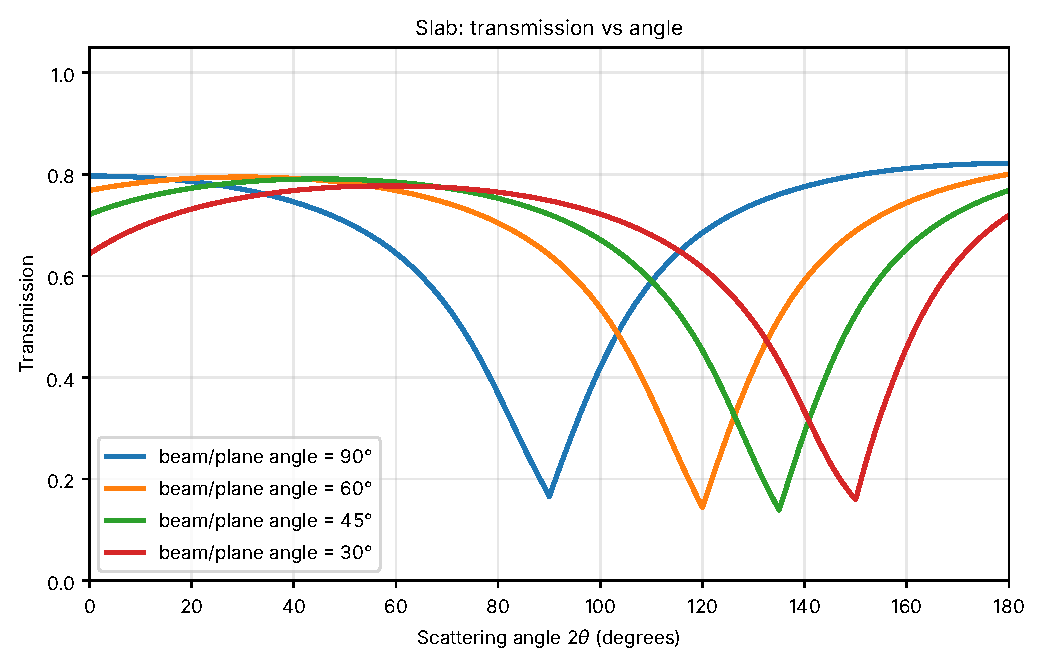
\includegraphics[width=0.8\textwidth]{fig_transmission_slab}
  \caption{Slab: transmission versus $\twotheta$ for four orientations of the sample (angle between the beam and the plane of the
  slab). The minimum follows the direction parallel to the layers.}
  \label{fig:tslab}
\end{figure}

\textbf{Cylinder.} The transmission of the cylinder (Figure~\ref{fig:tcyl}) is smooth and has no minimum: there is no direction along which the path
is especially long. Particles scattered backwards leave through the side from which the beam arrived, crossing less material, so $T$
grows with the angle.

\begin{figure}[ht]
  \centering
  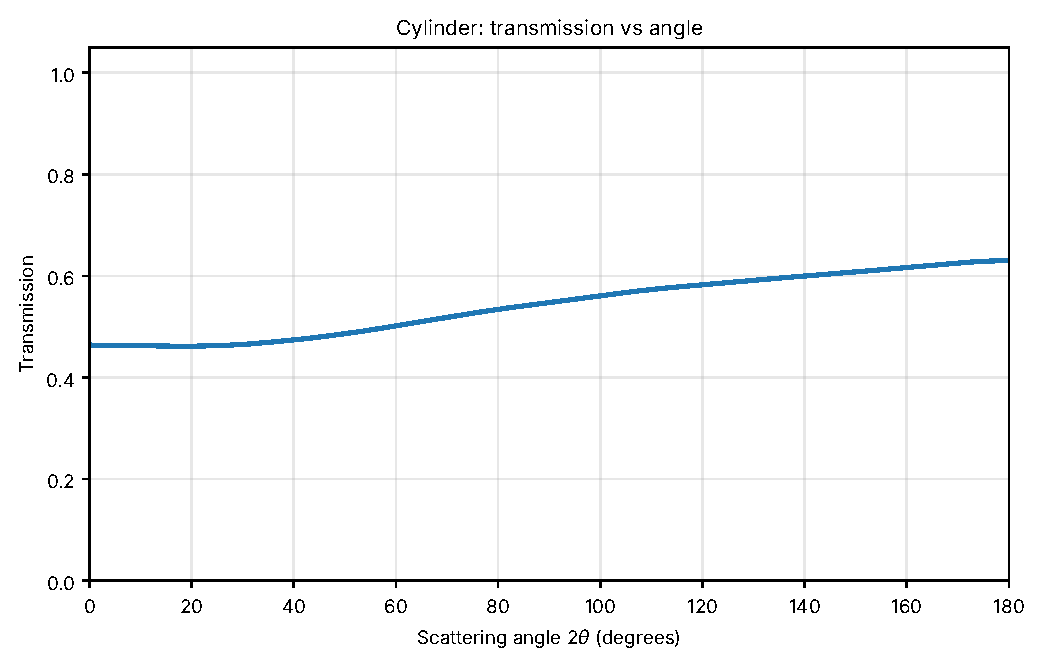
\includegraphics[width=0.8\textwidth]{fig_transmission_cylinder}
  \caption{Cylinder: transmission versus $\twotheta$ (the beam illuminates the whole cylinder, which has a diameter of 9~mm).}
  \label{fig:tcyl}
\end{figure}
